% Network architecture of JetAssignmentTransformer (src/model.py), 7-jet / ISR mode.
% Build: xelatex architecture.tex  (from docs/figures/; uses the bundled EB Garamond)
\documentclass[border=8pt]{standalone}
\usepackage{fontspec}
\setmainfont{EBGaramond12}[
  Path=../../assets/fonts/ebgaramond/,
  Extension=.otf,
  UprightFont=*-Regular, ItalicFont=*-Italic, BoldFont=*-Bold,
  Numbers=Lining]
\usepackage[italic]{mathastext}
\usepackage{amsmath,amssymb}
\usepackage{tikz}
\usetikzlibrary{arrows.meta,positioning,calc,backgrounds}

\definecolor{ink}{gray}{0.12}
\definecolor{quiet}{gray}{0.45}
\definecolor{rule}{gray}{0.55}
\definecolor{cell}{gray}{0.88}
\definecolor{slab}{RGB}{120,140,170}
\definecolor{tokfill}{RGB}{214,221,232}
\definecolor{cISR}{RGB}{196,88,40}
\definecolor{cG1}{RGB}{70,120,175}
\definecolor{cG2}{RGB}{90,150,100}

\tikzset{
  >={Stealth[length=4pt,width=3pt]},
  every node/.style={text=ink, font=\small},
  tok/.style={draw=ink!70, line width=0.4pt, minimum size=0.34cm, inner sep=0pt},
  layer/.style={draw=ink!70, fill=white, line width=0.45pt, rounded corners=2pt,
    minimum height=0.62cm, minimum width=2.0cm, align=center, inner sep=2pt},
  lbl/.style={font=\footnotesize, text=quiet},
  flow/.style={->, draw=ink!60, line width=0.5pt},
  ctx/.style={->, draw=cISR!80, line width=0.5pt, dash pattern=on 2.5pt off 1.5pt},
}
\newcommand{\h}{\mathbf h}
\newcommand{\g}{\mathbf g}

\begin{document}
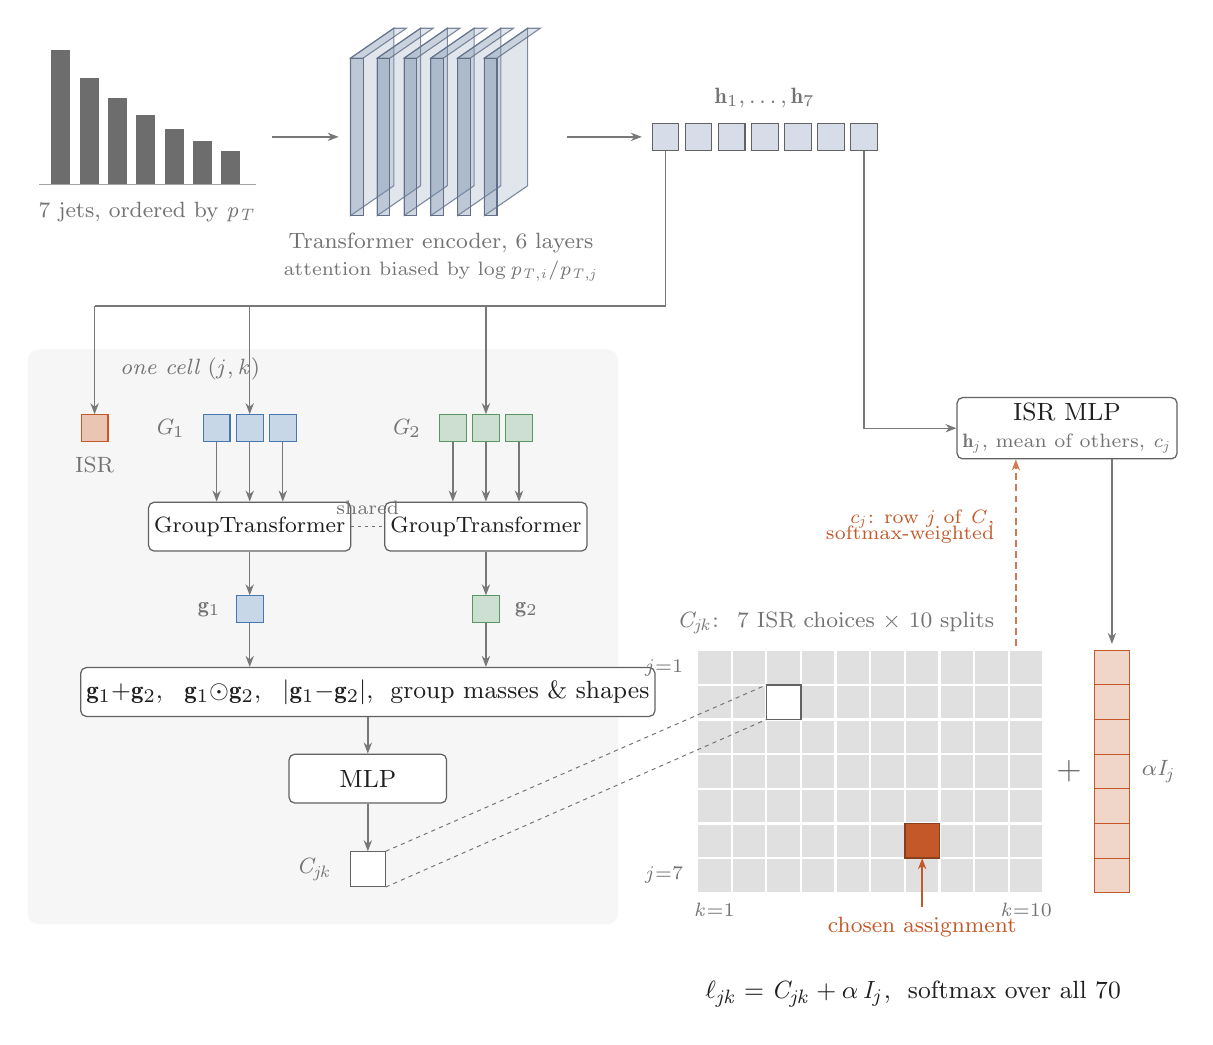
\begin{tikzpicture}[x=1cm,y=1cm]

% =====================================================================
% 1. jets, drawn as pT-ordered bars
% =====================================================================
\foreach \i/\ht in {1/1.7, 2/1.35, 3/1.1, 4/0.88, 5/0.7, 6/0.55, 7/0.42} {
  \fill[ink!65] ({0.2+(\i-1)*0.36},10.3) rectangle ++(0.24,\ht);
}
\draw[ink!40, line width=0.4pt] (0.05,10.3) -- (2.8,10.3);
\node[lbl, align=center] at (1.42,9.95) {7 jets, ordered by $p_T$};

% =====================================================================
% 2. Transformer encoder: six identical translucent layers
% =====================================================================
\def\dx{0.55} \def\dy{0.38}
\foreach \s in {0,...,5} {
  \pgfmathsetmacro{\x}{4.0+0.34*\s}
  \fill[slab, fill opacity=0.22, draw=slab!80!black, draw opacity=0.8, line width=0.4pt]
    (\x,9.9) -- ++(\dx,\dy) -- ++(0,2.0) -- ++(-\dx,-\dy) -- cycle;   % side
  \fill[slab, fill opacity=0.22, draw=slab!80!black, draw opacity=0.8, line width=0.4pt]
    (\x,11.9) -- ++(\dx,\dy) -- ++(0.16,0) -- ++(-\dx,-\dy) -- cycle; % top
  \fill[slab, fill opacity=0.35, draw=slab!80!black, line width=0.4pt]
    (\x,9.9) rectangle ++(0.16,2.0);                                  % front
}
\node[lbl, align=center] at (5.15,9.55) {Transformer encoder, 6 layers};
\node[lbl, align=center, font=\scriptsize] at (5.15,9.2) {attention biased by $\log p_{T,i}/p_{T,j}$};
\draw[flow] (3.0,10.9) -- (3.85,10.9);

% =====================================================================
% 3. jet embeddings
% =====================================================================
\foreach \i in {1,...,7} {
  \node[tok, fill=tokfill] (h\i) at ({8.0+(\i-1)*0.42},10.9) {};
}
\node[lbl, above=2pt of h4] {$\h_1,\dots,\h_7$};
\draw[flow] (6.75,10.9) -- (7.7,10.9);

% =====================================================================
% 4. zoom: what happens for one assignment (j, k)
% =====================================================================
\begin{scope}[on background layer]
  \fill[gray!7, rounded corners=4pt] (-0.1,0.9) rectangle (7.4,8.2);
\end{scope}
\node[lbl, anchor=west, font=\footnotesize\itshape] at (0.95,7.95) {one cell $(j,k)$};

\node[tok, fill=cISR!35, draw=cISR] (isr) at (0.75,7.2) {};
\node[lbl, below=2pt of isr] {ISR};
\foreach \k in {0,1,2} {
  \node[tok, fill=cG1!30, draw=cG1] (a\k) at ({2.3+\k*0.42},7.2) {};
  \node[tok, fill=cG2!30, draw=cG2] (b\k) at ({5.3+\k*0.42},7.2) {};
}
\node[lbl, left=3pt of a0] {$G_1$};
\node[lbl, left=3pt of b0] {$G_2$};

% gather: embeddings into the slots
\coordinate (bus) at (0,8.75);
\draw[draw=ink!60, line width=0.5pt] (h1.south) |- (0.75,8.75);
\draw[flow] (0.75,8.75) -- (isr.north);
\draw[flow] (a1.north |- 0,8.75) -- (a1.north);
\draw[flow] (b1.north |- 0,8.75) -- (b1.north);

\node[layer, font=\footnotesize] (gt1) at (2.72,5.95) {GroupTransformer};
\node[layer, font=\footnotesize] (gt2) at (5.72,5.95) {GroupTransformer};
\draw[draw=quiet, line width=0.4pt, dash pattern=on 1pt off 1.5pt] (gt1.east) -- (gt2.west)
  node[midway, above=1pt, lbl, font=\scriptsize] {shared};
\foreach \k in {0,1,2} {
  \draw[flow] (a\k.south) -- (a\k.south |- gt1.north);
  \draw[flow] (b\k.south) -- (b\k.south |- gt2.north);
}

\node[tok, fill=cG1!30, draw=cG1] (g1) at (2.72,4.9) {};
\node[tok, fill=cG2!30, draw=cG2] (g2) at (5.72,4.9) {};
\node[lbl, left=2pt of g1] {$\g_1$};
\node[lbl, right=2pt of g2] {$\g_2$};
\draw[flow] (gt1) -- (g1);
\draw[flow] (gt2) -- (g2);

\node[layer, minimum width=5.6cm] (sym) at (4.22,3.85)
  {$\g_1{+}\g_2,\ \ \g_1{\odot}\g_2,\ \ |\g_1{-}\g_2|,\ \ $group masses \& shapes};
\draw[flow] (g1) -- (g1 |- sym.north);
\draw[flow] (g2) -- (g2 |- sym.north);

\node[layer] (gmlp) at (4.22,2.75) {MLP};
\draw[flow] (sym) -- (gmlp);
\node[tok, fill=white, draw=ink!70, minimum size=0.44cm] (Cjk) at (4.22,1.6) {};
\node[lbl, left=3pt of Cjk] {$C_{jk}$};
\draw[flow] (gmlp) -- (Cjk);

% =====================================================================
% 5. the 70 assignments as a 7 x 10 grid, plus the ISR score column
% =====================================================================
\def\cs{0.44}
\def\gx{8.4} \def\gy{1.3}
\def\ix{13.45}

\fill[cell] (\gx,\gy) rectangle ++({10*\cs},{7*\cs});
\begin{scope}[shift={(\gx,\gy)}] \draw[white, line width=0.8pt] (0,0) grid[step=\cs] ({10*\cs},{7*\cs}); \end{scope}
\node[lbl, anchor=south] at ({\gx+4*\cs},{\gy+7*\cs+0.08}) {$C_{jk}$: \ 7 ISR choices $\times$ 10 splits};
\foreach \r in {1,7} { \node[lbl, font=\scriptsize, anchor=east] at ({\gx-0.05},{\gy+(7-\r+0.5)*\cs}) {$j{=}\r$}; }
\foreach \c in {1,10} { \node[lbl, font=\scriptsize] at ({\gx+(\c-0.5)*\cs},{\gy-0.22}) {$k{=}\c$}; }

% ISR score column, added to every column of the grid
\foreach \r in {1,...,7} { \fill[cISR!25] (\ix,{\gy+(7-\r)*\cs}) rectangle ++(\cs,\cs); }
\begin{scope}[shift={(\ix,\gy)}] \draw[cISR, line width=0.4pt] (0,0) grid[step=\cs] (\cs,{7*\cs}); \end{scope}
\draw[cISR, line width=0.4pt] (\ix,\gy) rectangle ++(\cs,{7*\cs});
\node[font=\large, text=ink!70] at ({(\gx+10*\cs+\ix)/2},{\gy+3.5*\cs}) {$+$};
\node[lbl, right=1pt] at ({\ix+\cs},{\gy+3.5*\cs}) {$\alpha I_j$};

% the cell zoomed into on the left (j = 2, k = 3)
\coordinate (zc) at ({\gx+2*\cs},{\gy+5*\cs});
\fill[white] (zc) rectangle ++(\cs,\cs);
\draw[ink!70, line width=0.5pt] (zc) rectangle ++(\cs,\cs);
\draw[quiet, line width=0.35pt, dash pattern=on 1.5pt off 1.5pt]
  (Cjk.north east) -- ($(zc)+(0,\cs)$)  (Cjk.south east) -- (zc);

% chosen assignment after the softmax (j = 6, k = 7)
\coordinate (best) at ({\gx+6*\cs},{\gy+1*\cs});
\fill[cISR] (best) rectangle ++(\cs,\cs);
\draw[cISR!70!black, line width=0.5pt] (best) rectangle ++(\cs,\cs);
\draw[<-, draw=cISR, line width=0.5pt] ($(best)+(\cs/2,0)$) -- ++(0,-0.62)
  node[below, text=cISR, font=\footnotesize] {chosen assignment};

\node[anchor=north] at ({(\gx+\ix+\cs)/2},0.3)
  {$\ell_{jk}=C_{jk}+\alpha\,I_j$, \ softmax over all 70};

% =====================================================================
% 6. ISR head
% =====================================================================
\node[layer, minimum width=2.7cm, align=center] (imlp) at (13.1,7.2)
  {ISR MLP\\[-1pt]{\scriptsize\color{quiet}$\h_j$, mean of others, $c_j$}};
\draw[flow] (h7.south) |- (imlp.west);
\draw[flow] ({\ix+\cs/2},0 |- imlp.south) -- ({\ix+\cs/2},{\gy+7*\cs+0.08});
% grouping quality back into the ISR head
\draw[ctx] (12.45,{\gy+7*\cs+0.05}) -- (12.45,0 |- imlp.south);
\node[font=\scriptsize, text=cISR, anchor=east, align=right] at (12.3,5.95)
  {$c_j$: row $j$ of $C$,\\[-2pt]softmax-weighted};

\end{tikzpicture}
\end{document}
